\documentclass[11pt,a4paper]{article}
\usepackage[utf8]{inputenc}
\usepackage[T1]{fontenc}
\usepackage{lmodern}
\usepackage[margin=2.2cm]{geometry}
\usepackage{amsmath,amssymb,amsthm}
\usepackage{booktabs}
\usepackage{array}
\usepackage{longtable}
\usepackage{enumitem}
\usepackage{tikz}
\usetikzlibrary{positioning,arrows.meta,calc}
\usepackage[hidelinks]{hyperref}

\setlist{itemsep=2pt,topsep=3pt}
\setlength{\parindent}{0pt}
\setlength{\parskip}{6pt}
\raggedright

\newtheorem{proposition}{Proposition}
\newtheorem{corollary}{Corollary}

\newcommand{\strat}[1]{\texttt{#1}}
\newcommand{\Ddecl}{D^{\mathrm{decl}}_t}
\newcommand{\Dobs}{D^{\mathrm{obs}}_t}
\newcommand{\Trep}{T^{\mathrm{rep}}(\Delta)}
\newcommand{\Tdiv}{T^{\mathrm{div}}(\Delta)}
\newcolumntype{L}[1]{>{\raggedright\arraybackslash}p{#1}}

\title{Replay first: which evals to run after a change,\\ in what order, and when to stop}
\date{}

\begin{document}
\maketitle
\vspace{-1.5cm}

\begin{abstract}
\noindent Every eval of an LLM agent system calls the model, so rerunning the suite after each change costs the
whole suite in tokens. \emph{Replay first} records the model's answers once. After a change it reruns every test
on those answers, without the model: a test that asks the model nothing new gets its outcome for free, and only
the other tests are run, in an order that brings a failure early and with a stopping rule that bounds how often a
regression is missed. These pages give the method, its guarantee and the conditions the guarantee needs. The
measurements are in the paper.
\end{abstract}

\section{The problem}
\label{sec:problem}

An LLM agent system is made of agents (a model with a prompt, skills and tools), the harness code that runs them,
and configuration. A \emph{test}, or eval, sends the system a request and checks what it did: the final state, the
tool calls and the answer. Every test calls the model, so every test costs tokens.

The question is which tests to run after a change, in what order, and when to stop, so that we catch regressions
while paying as few tokens as possible.

\paragraph{The words we use.}
\begin{itemize}
  \item A \emph{change} $\Delta$ turns the current version $V_0$ into a new version $V_1$: an edited prompt or
        skill, a tool that works differently, a new setting.
  \item A model produces the outcome of a test, so we run each test several times on $V_0$; $f_t$ is the share of
        the runs of test $t$ that fail. The test \emph{passes on $V_0$} when $f_t < \frac12$.
  \item A test \emph{reveals} $\Delta$ when it passes on $V_0$ and fails on $V_1$; $\mathrm{Rev}(\Delta)$ is the
        set of such tests.
  \item $\Delta$ is a \emph{regression} when some test reveals it. The verdict on a change is \textsc{regression}
        or \textsc{clean}.
\end{itemize}

\paragraph{Two rules for every run.} Whatever the method, a run of tests after a change follows two rules:
\begin{itemize}
  \item a test the model already fails on $V_0$ ($f_t \ge \frac12$) is not run: it cannot reveal anything;
  \item the run stops at the first failure, since a test that passed on $V_0$ and fails on $V_1$ means a
        regression.
\end{itemize}

\paragraph{The answer, in three steps} (Figure~\ref{fig:flow}).
\begin{itemize}
  \item \textbf{Replay} (Sections~\ref{sec:replay} to~\ref{sec:gives}). We record the model's answers on $V_0$
        once. After a change, we rerun every test with those recorded answers in place of the model. A test that
        never asks the model anything new gets its outcome for free. A test that does ask something new is one
        the change \emph{reaches}, and only those need the model.
  \item \textbf{Order} (Section~\ref{sec:order}). A strategy puts the reached tests in an order, the likeliest to
        fail first.
  \item \textbf{Stop} (Section~\ref{sec:stop}). A stopping rule may call the change clean before every reached
        test has run, with a threshold set on past changes so that the share of missed regressions stays under a
        target we choose. A coverage floor makes sure a clean verdict leaves no changed component and no release
        blocker untested.
\end{itemize}
A day's changes can also be tested together, as one batch; the replay then narrows a failure down to the changes
that can have caused it (Section~\ref{sec:day}).

\paragraph{An example.} Suppose a change edits the code of one tool. The replay reruns every test on $V_1$ without
the model. A test that never calls the tool, or calls it where it behaves as before, sends the same requests as on
$V_0$: it replays to the end and costs nothing. A test in which the tool now returns something else sends a
request that was never recorded: the change reaches it. The reached tests then run with the model, in a strategy's
order. The first failure ends the run with a regression; if all pass, or the stopping rule stops the run, the
change is clean.

\begin{figure}[h]
\centering
\resizebox{\textwidth}{!}{%
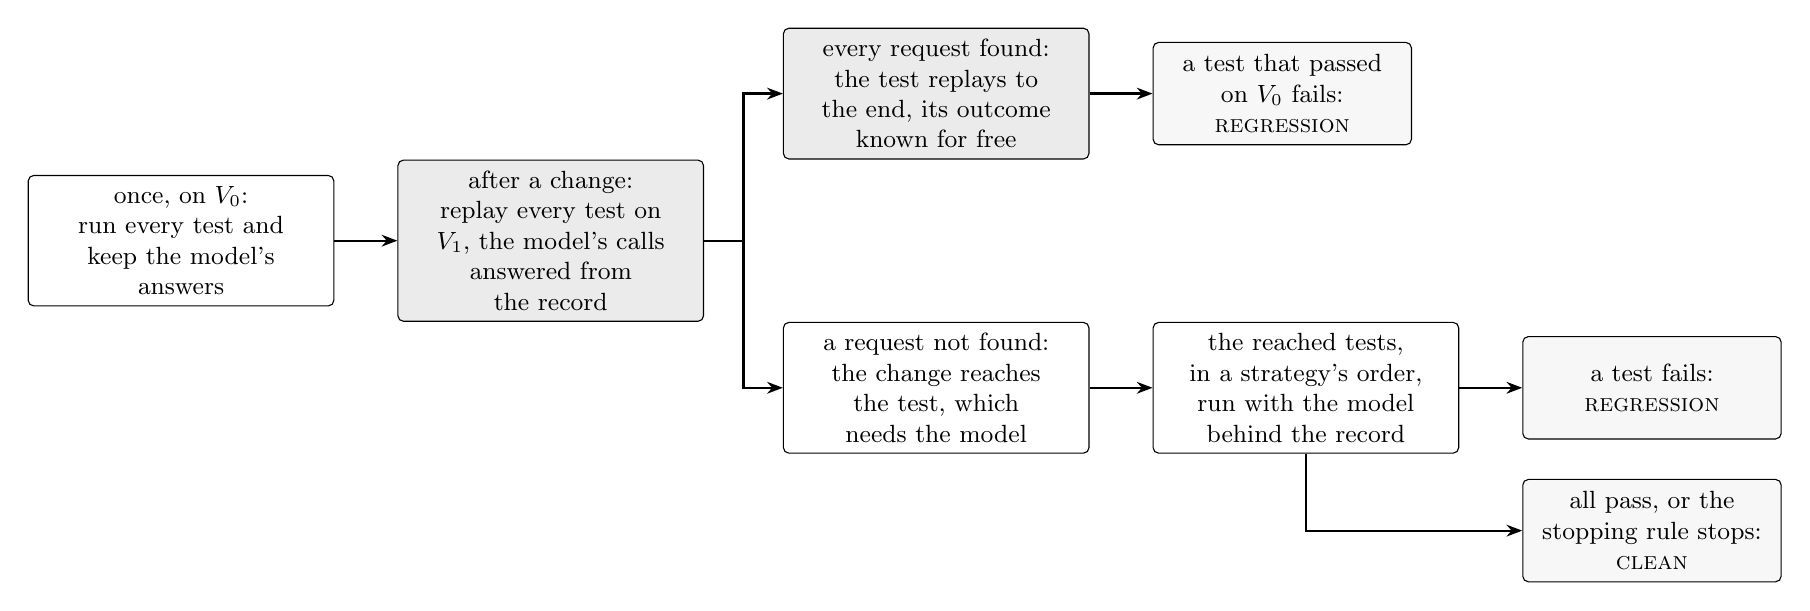
\begin{tikzpicture}[
  node distance=5mm and 8mm,
  box/.style={draw, rounded corners=2pt, align=center, font=\small, inner sep=4pt, minimum height=13mm,
    text width=36mm},
  free/.style={box, fill=black!8},
  verdict/.style={box, fill=black!3, text width=30mm},
  arr/.style={-{Stealth[length=2mm]}, thick}
]
\node[box] (rec) {once, on $V_0$:\\run every test and\\keep the model's\\answers};
\node[free, right=of rec] (rep) {after a change:\\replay every test on\\$V_1$, the model's calls\\answered from the record};
\node[free, above right=0mm and 10mm of rep] (end) {every request found:\\the test replays to\\the end, its outcome\\known for free};
\node[box, below right=0mm and 10mm of rep] (div) {a request not found:\\the change reaches\\the test, which\\needs the model};
\node[verdict, right=of end] (reg0) {a test that passed\\on $V_0$ fails:\\\textsc{regression}};
\node[box, right=of div] (run) {the reached tests,\\in a strategy's order,\\run with the model\\behind the record};
\node[verdict, right=of run] (reg) {a test fails:\\\textsc{regression}};
\node[verdict, below=of reg] (cl) {all pass, or the\\stopping rule stops:\\\textsc{clean}};
\draw[arr] (rec) -- (rep);
\draw[arr] (rep.east) -- ++(5mm,0) |- (end.west);
\draw[arr] (rep.east) -- ++(5mm,0) |- (div.west);
\draw[arr] (end) -- (reg0);
\draw[arr] (div) -- (run);
\draw[arr] (run) -- (reg);
\draw[arr] (run.south) |- (cl.west);
\end{tikzpicture}}
\caption{The flow after a change. Grey boxes make no model call.}
\label{fig:flow}
\end{figure}

\section{How the replay works}
\label{sec:replay}

\paragraph{A run, written down.} A run of a test is a conversation between the model and code. By \emph{code} we
mean everything that is not the model: the harness, the tools and the services behind them, the starting data, and
the test's checks. The code builds a \emph{request}, the model returns an \emph{answer}, the code acts on it (it
runs the tool the model asked for, say) and builds the next request, until the test's checks give the outcome.
For test $t$ on version $V$, with model $M$:
\[
  q_1 = g^t_V(), \qquad a_i = M(q_i), \qquad q_{i+1} = g^t_V(a_1, \dots, a_i), \qquad
  X_t(V) = h^t_V(a_1, \dots, a_n).
\]
\begin{itemize}
  \item A request $q_i$ is everything the model sees in that call: the system prompt, the messages so far
        including every tool result, the tools on offer, and the decoding settings. Calls to a judge model that
        grades the answer are requests too.
  \item $g^t_V$ is the code of $V$ running up to the next call, and $h^t_V$ the code running to the end and
        applying the test's checks.
  \item $X_t(V)$ is the outcome, pass or fail.
\end{itemize}

\paragraph{The cassette.} We run the suite on $V_0$ and keep every answer under the request that produced it. This
store is the \emph{cassette}: $Q_0$ is the set of requests it holds and $A_0(q)$ the answer kept for $q$.
\begin{itemize}
  \item A request is looked up by a hash of all of it, so two requests match only if they are identical.
  \item When repeated runs gave one request different answers, the most frequent is kept.
  \item Tool-call ids that a server makes up are first numbered by order of appearance, so that they do not break
        the match.
\end{itemize}

\paragraph{Replaying a test.} To replay test $t$ on $V_1$, we run it with $A_0$ in place of $M$. The code is the
code of $V_1$ and runs as it is; only the model's answers come from the cassette (Figure~\ref{fig:run}). One of two
things happens:
\begin{itemize}
  \item every request is in $Q_0$. The run finishes without the model, with outcome $\hat{X}_t(V_1)$, and $t$
        \emph{replays to the end}. These tests form $\Trep$;
  \item the run reaches a request $q \notin Q_0$, its \emph{divergence point}. The cassette has no answer, the
        replay of $t$ stops there, and $t$ \emph{diverges}. These tests form $\Tdiv$, the tests the change
        \emph{reaches}.
\end{itemize}
The replay makes no model call, so it costs no tokens and takes only the time the code needs.

\begin{figure}[h]
\centering
\resizebox{\textwidth}{!}{%
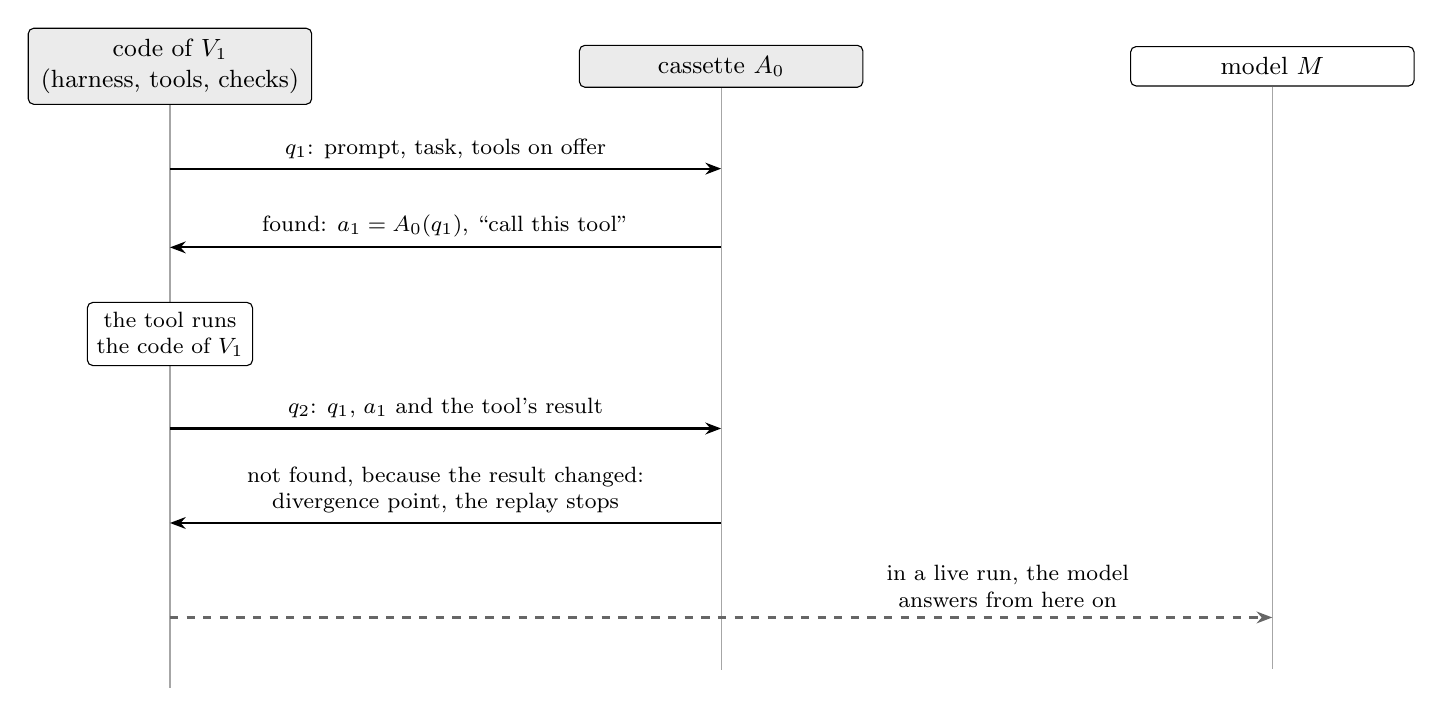
\begin{tikzpicture}[
  font=\small,
  lane/.style={draw, rounded corners=2pt, fill=black!8, inner sep=4pt, align=center, minimum width=36mm},
  msg/.style={-{Stealth[length=2mm]}, thick},
  live/.style={-{Stealth[length=2mm]}, thick, dashed, black!60},
  lbl/.style={above, align=center, font=\footnotesize}
]
\node[lane] (code) at (0,0) {code of $V_1$\\(harness, tools, checks)};
\node[lane] (cas) at (7,0) {cassette $A_0$};
\node[lane, fill=white] (mod) at (14,0) {model $M$};
\foreach \n in {code,cas,mod} \draw[black!35] (\n.south) -- ++(0,-7.4);
\draw[msg] (0,-1.3) -- node[lbl] {$q_1$: prompt, task, tools on offer} (7,-1.3);
\draw[msg] (7,-2.3) -- node[lbl] {found: $a_1 = A_0(q_1)$, ``call this tool''} (0,-2.3);
\node[draw, fill=white, rounded corners=2pt, align=center, font=\footnotesize] at (0,-3.4)
  {the tool runs\\the code of $V_1$};
\draw[msg] (0,-4.6) -- node[lbl] {$q_2$: $q_1$, $a_1$ and the tool's result} (7,-4.6);
\draw[msg] (7,-5.8) -- node[lbl] {not found, because the result changed:\\divergence point, the replay stops} (0,-5.8);
\draw[live] (0,-7.0) -- node[lbl, pos=0.76, text=black] {in a live run, the model\\answers from here on} (14,-7.0);
\end{tikzpicture}}
\caption{Replaying one test. Only the model's answers come from the cassette. Tools and checks run the code of
$V_1$, and a tool's result is part of the next request, so a tool that now returns something else makes the test
diverge.}
\label{fig:run}
\end{figure}

\paragraph{Where a change shows.} Since $g$ and $h$ are the code of $V_1$, a change shows wherever it alters what
the model sees or what the code does with the answers. By what the change alters:
\begin{itemize}
  \item \textbf{what an agent gets up front} (its prompt, its skills, its tools and their descriptions, its task):
        the first request of that agent's conversation is new, and the test diverges there;
  \item \textbf{a tool's code, a service, the starting data, or a setting the code reads:} a tool result differs
        whenever the test's call hits the changed behaviour. The next request is then new, and the test diverges
        there;
  \item \textbf{only state the model never reads:} the test replays to the end, and its checks fail it;
  \item \textbf{none of this:} the run is as it was on $V_0$, and the test replays to its recorded outcome.
\end{itemize}
Tools are never answered from the cassette: they always run the new code.

\paragraph{This is not prompt caching.} Model providers and servers offer \emph{prompt caching}, also called
prefix caching: they keep the computation for a prompt prefix they have seen before, and still generate a new
answer. That makes a call cheaper and faster, but every call is still made. A request the cassette holds makes no
call at all.

\section{When the replayed outcome is the real one}
\label{sec:conditions}

The replay stands in for the model, so it tells us about a real run only if two conditions hold.
\begin{itemize}
  \item \textbf{Condition R.} With the model served the way we serve it, the same request always gets the same
        answer: $M(q) = A_0(q)$ for every $q \in Q_0$.
  \item \textbf{Condition D.} Given the answers, the code is deterministic: $g^t_V$ and $h^t_V$ read no clock,
        draw no random numbers, and call no outside service whose reply can change.
\end{itemize}

\begin{proposition}
\label{prop:replay}
Under R and D, a test in $\Trep$, run on $V_1$ with the real model, sends the requests of its replay and gets the
same answers, so $X_t(V_1) = \hat{X}_t(V_1)$. A test in $\Tdiv$ matches its replay up to its divergence point.
\end{proposition}

\begin{proof}
By induction on $i$. The first requests match, because both runs execute the code of $V_1$, which is
deterministic by D. If the $i$-th requests match and are in $Q_0$, the model answers $M(q_i) = A_0(q_i)$ by R, so
the $i$-th answers match, and by D so do the next requests. A test in $\Trep$ ends with the same answers, and
$h^t_{V_1}$ turns them into one outcome. A test in $\Tdiv$ matches up to its first request outside $Q_0$.
\end{proof}

\begin{corollary}
\label{cor:safe}
Under R and D, every test that reveals the change either diverges or fails in the replay:
$\mathrm{Rev}(\Delta) \subseteq \Tdiv \cup \{t \in \Trep : \hat{X}_t(V_1) = \text{fail}\}$.
\end{corollary}

\begin{proof}
A test in $\Trep$ that reveals the change fails on $V_1$, and by the proposition its replay has the same outcome.
\end{proof}

Neither condition is taken on trust.

\paragraph{Checking D.} D is a property of the system under test: its services are simulated or recorded, it reads
no clock and draws no random numbers, and it derives its keys from the operation. The check is free: replayed
against its own cassette, $V_0$ must reach the end of every test with the recorded outcome.

\paragraph{Checking R.} R is a property of the model and of the way it is served. Even with deterministic decoding
(temperature 0, always the most likely token), a GPU server is not exact to the bit: the batch a request shares
with other requests, and the server's prefix cache, change the floating-point arithmetic and now and then a token.
We measure R with the \emph{empty change}: $V_0$ run again exactly the way a changed version is run, and compared
with the cassette at three levels:
\begin{itemize}
  \item \emph{requests}: how many get an answer other than the cassette's;
  \item \emph{runs}: how many tests have a run that differs from the recorded one;
  \item \emph{outcomes}: how many tests pass or fail otherwise.
\end{itemize}
An answer can be worded differently without the run taking another path, and a run can differ without its outcome
changing. What the replay claims is a test's outcome, so the third level is the one it needs.

\paragraph{In practice.}
\begin{itemize}
  \item When exact answers matter, serve the model without its prefix cache and with one test at a time per
        server, and confirm it with the empty change.
  \item A cassette is valid only for the model and the serving setup it was recorded with. A hosted model can
        change without notice; running the empty change from time to time tells us when to record again.
\end{itemize}

\section{What the replay gives}
\label{sec:gives}

Under R and D, the replay settles part of the verdict before any model call, and says which tests the rest needs:

\begin{center}
\begin{tabular}{@{}L{7.4cm}L{8.6cm}@{}}
\toprule
the replay finds & so \\
\midrule
$t \in \Trep$ passes & $t$ passes on $V_1$; no need to run it \\
\addlinespace
$t \in \Trep$ fails, and $t$ passes on $V_0$ & regression, before any model call \\
\addlinespace
$\Tdiv$ is empty, and no such failure & clean: no test can tell $V_1$ from $V_0$ \\
\addlinespace
$t \in \Tdiv$ & $t$ needs the model, for its requests outside $Q_0$ \\
\addlinespace
every $t \in \Tdiv$ that passes on $V_0$ is run, and passes & clean, with nothing the change reaches left
  untested \\
\bottomrule
\end{tabular}
\end{center}

\paragraph{What a reached test costs.} A reached test runs with the model behind the cassette: any request already
in $Q_0$ is answered from the cassette, and only new requests go to the model. Its cost is
\[
  c_\Delta(t) = \sum_{q \,\in\, \mathrm{run}(t, V_1),\ q \notin Q_0} \mathrm{tokens}(q).
\]
Before any model call, the replay bounds it from above by the tokens of $t$ after its divergence point. The bound
is loose because, after that point, a run may still send requests that are in $Q_0$, such as the turn of an agent
the change does not touch. Strategies plan with the bound.

\paragraph{Compared with a plain answer cache.} A cache of answers in front of the model gives the same saving to
any rerun of the suite, with no method at all: the whole suite, rerun through the cache, pays only for the new
requests and finds every regression. That is the cost to beat. Replay first can pay less in three ways:
\begin{itemize}
  \item the tests the model already fails are not run;
  \item a run ends at its first failure, so the order of the reached tests decides what a regression costs
        (Section~\ref{sec:order});
  \item a stopping rule ends a run before every reached test has run, which decides what a change that breaks
        nothing costs (Section~\ref{sec:stop}).
\end{itemize}

\section{Ordering the reached tests}
\label{sec:order}

The reached tests are a small suite, and putting them in order is classic test prioritization. A good order brings
a revealing test early, because the run ends at the first failure. The strategies differ in what they read.

\paragraph{What a strategy can read.} A \emph{component} is a part of the system a change can touch: a function or
line of code, a tool and its description, a skill's procedure or text, a field of an agent, a setting, the
starting data. $C(\Delta)$ is the set of components the change touches. For each test $t$ we know:
\begin{itemize}
  \item $c(t)$, its cost in tokens on $V_0$, and $\rho_t$, a risk weight its author gave it;
  \item $\Ddecl$, the components its author declared it depends on;
  \item $\Dobs$, the components its runs on $V_0$ actually exercised, from traces and code coverage, and
        $\phi_t(c)$, the share of its runs that exercised component $c$.
\end{itemize}
A component matches a test by one rule used everywhere: a changed function or line matches the tests that ran it, a
skill the tests that loaded it, a tool the tests it was offered to, a setting the tests that read it.

\paragraph{The baselines.} The table lists them by what they read. Two scores recur in it: the \emph{overlap} $a_t$
of a test with the change, and $e_t$, which is 1 when $t$ ran a changed line and 0 otherwise.

{\small
\begin{longtable}{@{}L{2.5cm}L{2.9cm}L{10.3cm}@{}}
\toprule
it reads & strategy & the order \\
\midrule
\endhead
\bottomrule
\endlastfoot
nothing & \strat{random} & a random permutation, as a reference \\
\addlinespace
declared dependencies & \strat{declared} &
  classic selection: the tests with $\Ddecl \cap C(\Delta) \neq \emptyset$, by $\rho_t$, then by the overlap
  $a_t = |\Ddecl \cap C(\Delta)|$, both descending, then cheapest first \\
\addlinespace
observed dependencies & \strat{observed} &
  the tests with $\Dobs \cap C(\Delta) \neq \emptyset$, by $a_t\, \rho_t / c(t)$ descending, where the overlap
  is $a_t = \sum_{c \in C(\Delta) \cap \Dobs} \phi_t(c)$ \\
\addlinespace
 & \strat{cost\_aware} &
  the whole suite, by $\rho_t\, (\beta_0 + a_t + e_t)\, (1 + f_t) / c(t)$ descending; the small constant $\beta_0$
  keeps the tests the change does not touch in the order \\
\addlinespace
the text of the diff and of the test & \strat{ir\_tfidf} &
  by the TF-IDF similarity of the diff and the test's text (name, request, expected outcome): two texts are close
  when they share words that are rare across the tests \\
\addlinespace
past changes & \strat{history\_ml} &
  by $p_t\, \rho_t / c(t)$ descending, where $p_t$ is the probability that $t$ reveals the change, from a logistic
  regression (a linear model that outputs a probability) fitted on pairs (past change, test); its features are
  the change's impact on the test by kind of component, and the test's cost, risk and shape \\
\addlinespace
the results so far & \strat{casper\_slices} &
  adapted from CASPER: it groups the tests that behave alike on $V_0$ with k-means, runs a few representatives of
  each group on $V_1$, then runs the groups whose failure rate moved the most \\
\addlinespace
 & \strat{risk\_aware\_ts} &
  adapted from Risk-Aware Adaptive Evaluation, a bandit with Thompson sampling: a logistic regression on the
  results so far estimates each test's chance to fail, a value $\theta_t$ is drawn at random around the estimate,
  and the test with the largest $\rho_t\, \theta_t$ runs next \\
\addlinespace
the replay only & \strat{cheapest} & by the cost bound of Section~\ref{sec:gives}, ascending \\
\addlinespace
 & \strat{late\_divergence} & by how late the change reaches the test, latest first \\
\end{longtable}
}

\paragraph{Our method, \strat{adaptive\_bayes}.} It keeps a probability for what the change broke, and recomputes
the order after every result.
\begin{enumerate}
  \item \textbf{Hypotheses.} A hypothesis $h \in \{0,1\}^{C(\Delta)}$ says which changed components are broken.
        Each component $c$ starts with a prior probability $\pi_c$ that depends on its kind: higher for code,
        skill procedures, settings and agent fields, lower for prompt wording, skill prose and tool descriptions.
  \item \textbf{What a result says.} A test passes only if it would pass on $V_0$ and no broken component makes it
        fail:
        \[ P(t \text{ fails} \mid h) = 1 - (1 - f_t) \prod_{c:\, h_c = 1} (1 - s_{tc}). \]
  \item \textbf{Sensitivity.} $s_{tc}$ is the chance that $t$ fails when $c$ is broken. Exercising a component is
        weak evidence by itself, so $s_{tc}$ is a product of four factors, kept between a floor and a ceiling.
        With $k$ the kind of $c$:
        \[ s_{tc} = \mathrm{clip}\big(r_k \cdot \ell_{tk} \cdot \phi_t(c) \cdot \mathrm{bonus}_t,\ s_{\min},\
           s_{\max}\big). \]
        \begin{itemize}
          \item $r_k$: how often the tests that touched past changes of kind $k$ revealed them;
          \item $\ell_{tk}$: how much better than the average test $t$ did on that kind;
          \item $\phi_t(c)$: how often the runs of $t$ on $V_0$ exercised $c$;
          \item $\mathrm{bonus}_t$: larger when the test's text is close to the diff, or its author declared the
                dependency.
        \end{itemize}
        The first two are learned from past changes, never from the change under test.
  \item \textbf{The next test.} After each result, Bayes' rule gives the \emph{posterior}, the probability of each
        hypothesis given the results so far. Its \emph{entropy} $H(h)$ measures how unsure we still are about
        what is broken. The next test is the one whose result is expected to lower that uncertainty the most per
        token, tilted by risk:
        \[ \arg\max_t\ \frac{H(h) - \mathbb{E}[H(h \mid X_t)]}{c(t)}\, \big(1 + \gamma(\rho_t - 1)\big). \]
  \item \textbf{Near-duplicates.} After a test passes, the sensitivity of the tests that behave just like it is
        multiplied by $\delta < 1$, since their passing would add little.
\end{enumerate}
The posterior also gives $P(\text{something is broken}) = 1 - P(h = \mathbf{0} \mid \text{results so far})$, which
is what the stopping rule of the next section reads.

\section{When to stop}
\label{sec:stop}

Without a stopping rule, \emph{clean} is the expensive verdict: giving it means running every reached test. A
stopping rule saves exactly there, and in exchange it has to say how often it is wrong.

\paragraph{The rule.} A stopping rule gives each test in its plan a value, $v_1 \ge v_2 \ge \dots$: how much
reason is left to keep going when that test's turn comes. The run stops with ``clean'' at the first value below a
threshold $\tau$. For \strat{adaptive\_bayes} the value is $P(\text{something is broken})$ before the test.

\paragraph{Setting the threshold.} We set $\tau$ on past regressions, with \emph{split conformal prediction}, a
technique that turns the ranks of past scores into a bound on the error rate (Figure~\ref{fig:stop}).
\begin{itemize}
  \item The \emph{score} $s(\Delta)$ of a past regression $\Delta$ is the value at the first test in the plan
        that reveals it. A threshold above the score would have stopped before that test and called $\Delta$
        clean.
  \item With $n$ past regressions and a target miss rate $\alpha$, the threshold is the $k$-th smallest score:
        \[ \tau = s_{(k)}, \qquad k = \lfloor \alpha (n + 1) \rfloor . \]
  \item A new regression is then called clean with probability at most $\alpha$, as long as past and new changes
        are \emph{exchangeable}, that is, drawn alike from the same pool of changes.
\end{itemize}

\paragraph{What the bound covers.}
\begin{itemize}
  \item It holds on average, over changes and over the sets of past regressions, and only for changes like the
        past ones.
  \item We set one threshold per group of changes: a skill's steps, text the model reads, an agent's tools and
        skills, the settings, the starting data, the code. A single threshold for all changes can meet the target
        on average while missing most regressions of one group.
\end{itemize}

\begin{figure}[h]
\centering
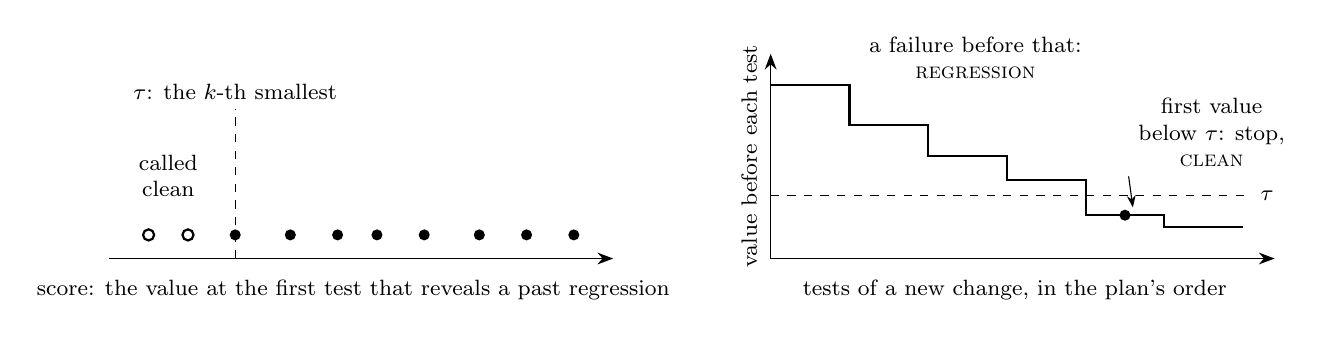
\begin{tikzpicture}[font=\footnotesize]
  % left: the scores of past regressions, and the threshold
  \draw[-{Stealth[length=2mm]}] (0,0) -- (6.4,0);
  \node[below, align=center] at (3.1,-0.15) {score: the value at the first test that reveals a past regression};
  \foreach \x in {0.5,1.0} \draw[thick] (\x,0.3) circle (2pt);
  \foreach \x in {1.6,2.3,2.9,3.4,4.0,4.7,5.3,5.9} \fill (\x,0.3) circle (2pt);
  \draw[dashed] (1.6,0) -- (1.6,1.9);
  \node[above, align=center] at (1.6,1.9) {$\tau$: the $k$-th smallest};
  \node[align=center] at (0.75,1.05) {called\\clean};
  % right: one new change, its plan and the stop
  \begin{scope}[xshift=8.4cm]
    \draw[-{Stealth[length=2mm]}] (0,0) -- (6.4,0);
    \draw[-{Stealth[length=2mm]}] (0,0) -- (0,2.6);
    \node[below] at (3.1,-0.15) {tests of a new change, in the plan's order};
    \node[rotate=90, above] at (-0.05,1.3) {value before each test};
    \draw[thick] (0,2.2) -- (1,2.2) -- (1,1.7) -- (2,1.7) -- (2,1.3) -- (3,1.3) -- (3,1.0) -- (4,1.0) -- (4,0.55)
      -- (5,0.55) -- (5,0.4) -- (6,0.4);
    \draw[dashed] (0,0.8) -- (6.1,0.8) node[right] {$\tau$};
    \fill (4.5,0.55) circle (2pt);
    \node[align=center] (stop) at (5.6,1.6) {first value\\below $\tau$: stop,\\\textsc{clean}};
    \draw[-{Stealth[length=1.5mm]}] (stop.south west) -- (4.6,0.65);
    \node[align=center] at (2.6,2.55) {a failure before that:\\\textsc{regression}};
  \end{scope}
\end{tikzpicture}
\caption{Setting and using the threshold. Left: each dot is a past regression of one group, placed at its score;
$\tau$ is the $k$-th smallest, and the regressions to its left are the ones the threshold would have called clean.
Right: on a new change, the run stops with clean at the first test whose value is below $\tau$, unless a test
fails first.}
\label{fig:stop}
\end{figure}

\paragraph{Properties.} Each test is tagged with the requirements it checks, taken from a catalog of
\emph{properties} (for example, ``a page is never published with broken links''). Some are \emph{mandatory}:
release blockers. From the components the change touches we know which properties it may affect, and a check
reports which affected properties it checked and which it did not.

\paragraph{The coverage floor.} A stopping rule decides when the evidence is strong enough, not what has been
looked at. The \emph{coverage floor} adds that: no ``clean'' before every changed component that some test
exercises, and every affected mandatory property that some test checks, has been covered. With $K$ the tests whose
outcome is already known (the replayed ones, and those already run) and $U_t$ what test $t$ covers of the change,
the floor is a cheapest set
\[
  F(\Delta) \subseteq \Tdiv \qquad \text{such that} \qquad \bigcup_{t \in F(\Delta) \cup K} U_t = \bigcup_{t \in
  \Tdiv \cup K} U_t ,
\]
found greedily, by the most uncovered items per token.
\begin{itemize}
  \item The floor runs just before a clean verdict, not first, so it costs nothing when a regression shows up
        earlier.
  \item It guarantees coverage, not detection: covering is not catching (Section~\ref{sec:minimal}). It goes
        under the stopping rule and does not replace it.
\end{itemize}

\section{Why not a fixed minimal set}
\label{sec:minimal}

The classic alternative is \emph{test-suite minimization}: pick once a small set of tests that still covers the
whole system, and run only that set after every change. With $U_t$ what test $t$ covers (the components it
exercises, or the properties it checks), this is a \emph{set cover} problem:
\[
  \min_{S \subseteq T} |S| \ \ \text{(or } \textstyle\sum_{t \in S} c(t)\text{)} \qquad \text{such that} \qquad
  \bigcup_{t \in S} U_t = \bigcup_{t \in T} U_t ,
\]
usually solved greedily, adding the test that covers the most of what is still uncovered (or the most per token).
Such a set misses regressions for two reasons:
\begin{itemize}
  \item \textbf{Covering is not catching.} A test covers a component when it exercises it, but it catches a broken
        component only if its checks look at exactly the behaviour that broke. A change that skips a permission
        check, for instance, is covered by every test that goes through that code, and caught only by the tests
        that exercise the case where the check should have stopped the action.
  \item \textbf{The set does not know the change.} A fixed set $S$ misses $\Delta$ exactly when
        $\mathrm{Rev}(\Delta) \cap S = \emptyset$. A regression that only one test reveals is caught only if that
        test happens to be in $S$, which was chosen before $\Delta$ existed.
\end{itemize}
Choosing per change avoids both. The replay picks, for each change, the tests through which it can reach the model,
and by Corollary~\ref{cor:safe}, running all of $\Tdiv$ and reading the outcomes of the others from the replay
misses no test that reveals the change. The coverage floor is the minimal set done per change: chosen among the
reached tests after the replay, and used as a floor under the stopping rule, not as the whole selection.

\section{A day of changes}
\label{sec:day}

A team merges many changes a day. Testing each one alone repeats the tests they share, and misses failures that
appear only when changes meet. Testing the day's changes together, as one \emph{batch}, avoids both, but a failing
test then does not say which change broke it. The replay helps at three moments.

\paragraph{Before any model call: the day's map.} Every change of the day is replayed alone, and so is the batch.
This gives the day's \emph{map}, which tests each change reaches, and it settles some changes at once:
\begin{itemize}
  \item a change that reaches no test and fails none in its replay needs no model at all, since no test can reveal
        it (Corollary~\ref{cor:safe}). If it was meant to change what the application does, the suite has no test
        for it, and the map shows that gap before anything runs;
  \item a change whose own replay fails a test that passes on $V_0$ is a regression, found with its culprit.
\end{itemize}

\paragraph{The run: once for the whole day.} The tests the batch reaches run once, with the model. A test that
several changes reach is paid for once, not once per change.

\paragraph{After a failure: the suspects.} When a test fails on the batch, the \emph{suspects} are the changes
whose own replay reaches that test or fails it. A change whose own replay runs the test to the end and passes
cannot make it fail on its own, and a change that makes the test fail by itself is always a suspect: that is
Corollary~\ref{cor:safe} applied to the change alone.
\begin{itemize}
  \item \textbf{One suspect:} it is the culprit, with no further run.
  \item \textbf{Several:} they are told apart by halving. Run the failing test with half of them, keep the half
        that still fails, and repeat: about $\log_2$ of their number of runs.
  \item \textbf{None,} or a halving that ends with no single change that fails the test: the failure needs the
        changes together, an \emph{interaction} that only the batch shows.
\end{itemize}

\section{Limits}

Besides conditions R and D:
\begin{itemize}
  \item \textbf{Exact matching is conservative.} A request that differs by one character, say a reworded prompt,
        sends the test to the model even if the meaning is the same. When every request carries one long shared
        prompt, editing it reaches every test and the replay saves nothing.
  \item \textbf{Clean means clean for this suite.} The replay says which existing tests can see the change. A
        regression that no test checks stays invisible, as with any test selection.
\end{itemize}

\section{Where it lives in the code}

In the order of these pages:
\begin{itemize}
  \item the replay: \texttt{traceeval replay-first}, \texttt{traceeval/experiment/replay\_first.py}; the cassette
        and the clients that answer from it: \texttt{traceeval/llm/cache.py};
  \item recording changes on the reached tests only: \texttt{traceeval mutants -{}-reached-only},
        \texttt{traceeval/experiment/runner.py::record\_mutants};
  \item the strategies: \texttt{traceeval/selection/};
  \item the stopping threshold: \texttt{traceeval/experiment/stopping.py};
  \item the coverage floor: \texttt{traceeval/experiment/coverage.py::coverage\_floor};
  \item checking one change live: \texttt{traceeval check <change> -{}-history <recording>}, with
        \texttt{-{}-miss-rate} for the threshold and \texttt{-{}-floor} for the coverage floor,
        \texttt{traceeval/experiment/check.py};
  \item a batch: the same check also prints the day's map and the suspects of a failing test,
        \texttt{traceeval/experiment/culprits.py}.
\end{itemize}

\end{document}
